\documentclass[tikz,border=5pt]{standalone}
\usepackage{tikz}
\usetikzlibrary{arrows.meta, positioning, fit}

\begin{document}

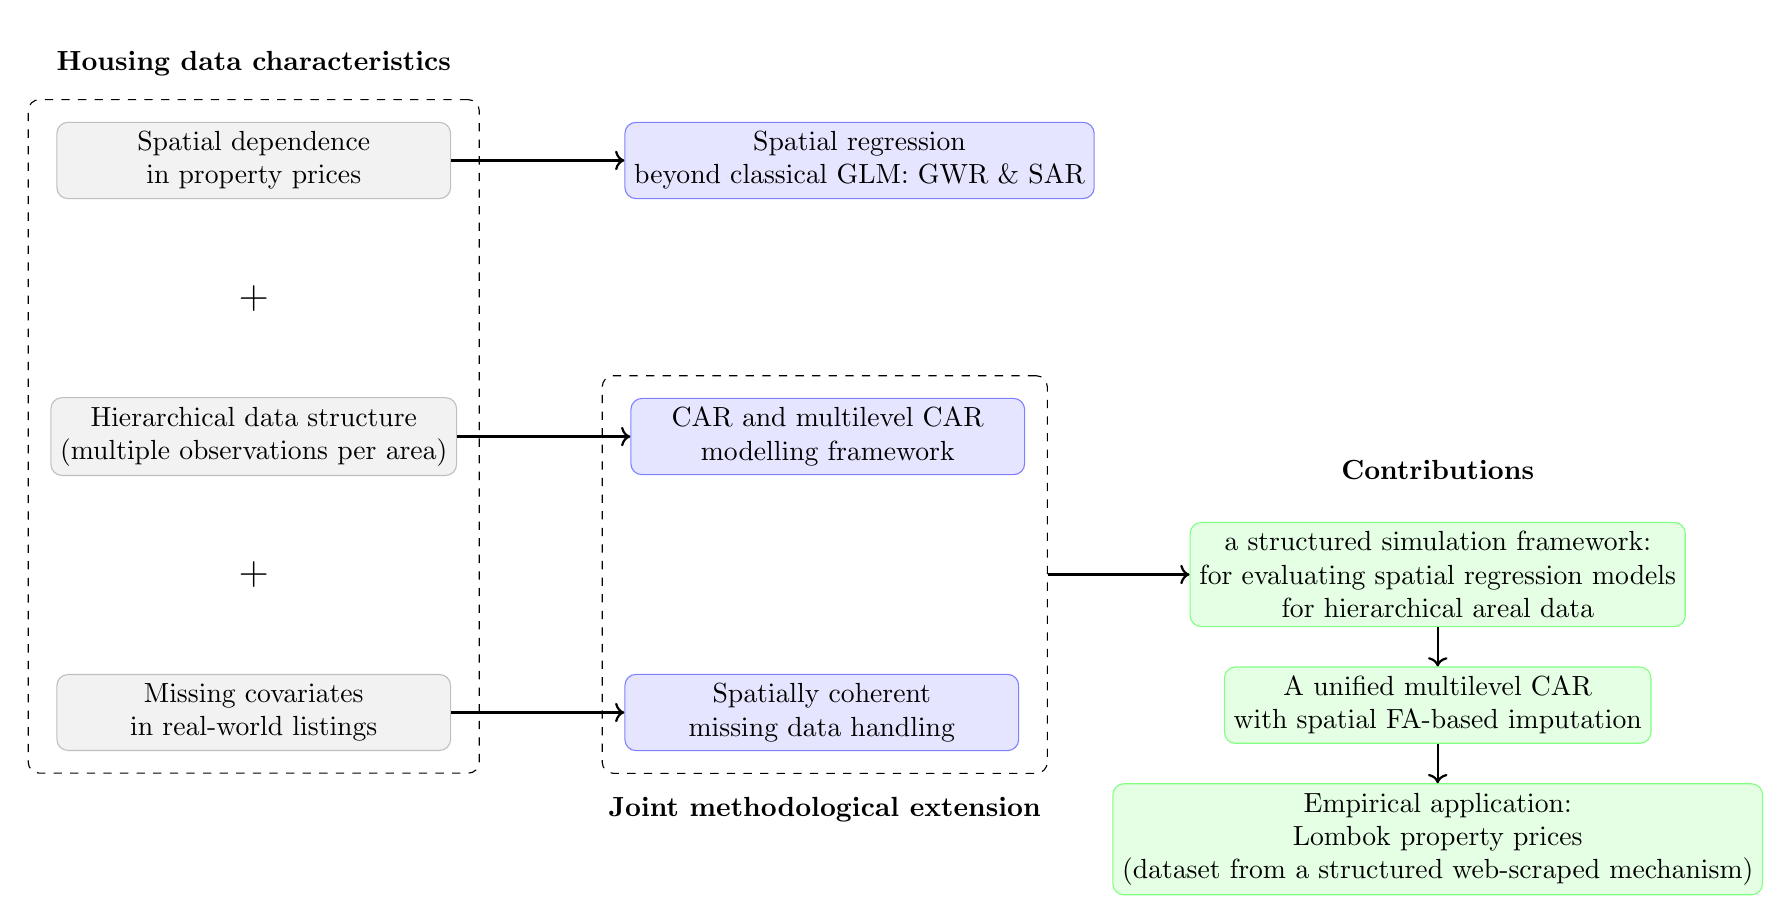
\begin{tikzpicture}[
    every node/.style={
        draw,
        rounded corners,
        align=center,
        minimum width=5.0cm,
        minimum height=9mm
    },
    arrow/.style={->, thick},
    node distance=8mm
]

% ------------------------
% Housing data characteristics (left)
% ------------------------
\node (d1) [fill=gray!10,
  draw=gray!50]
{Spatial dependence\\ in property prices};

\node[draw=none, below=of d1] (plus1) {\Large $+$};

\node (d2) [below=of plus1,
fill=gray!10,
  draw=gray!50]
{Hierarchical data structure\\ (multiple observations per area)};

\node[draw=none, below=of d2] (plus2) {\Large $+$};

\node (d3) [below=of plus2,
fill=gray!10,
  draw=gray!50]
{Missing covariates\\ in real-world listings};

% Dashed box for data characteristics
\node[
    draw,
    dashed,
    rounded corners,
    fit=(d1)(d2)(d3)(plus1)(plus2),
    inner sep=8pt,
    label=above:{\textbf{Housing data characteristics}}
] (databox) {};

% ------------------------
% Methodological directions (middle)
% ------------------------
\node (m1) [right=22mm of d1,
fill=blue!10,
  draw=blue!50]
{Spatial regression\\ beyond classical GLM: GWR \& SAR};

\node (m2) [right=22mm of d2,
fill=blue!10,
  draw=blue!50]
{CAR and multilevel CAR\\ modelling framework};

\node (m3) [right=22mm of d3,
fill=blue!10,
  draw=blue!50]
{Spatially coherent\\ missing data handling};

% Dashed box around joint extension
\node[
    draw,
    dashed,
    rounded corners,
    fit=(m2)(m3),
    inner sep=8pt,
    label=below:{\textbf{Joint methodological extension}}
] (methodbox) {};

% ------------------------
% Final contribution (right)
% ------------------------
\node (final) [
  right=18mm of methodbox,
  fill=green!10,
  draw=green!50,
  label={[label distance=2mm]above:{\textbf{Contributions}}}
]
{a structured simulation framework:\\ for evaluating spatial regression models\\
for hierarchical areal data};

% ------------------------
% Arrows
% ------------------------
\draw[arrow] (d1) -- (m1);
\draw[arrow] (d2) -- (m2);
\draw[arrow] (d3) -- (m3);

\draw[arrow] (methodbox) -- (final);

% ------------------------
% Empirical application (below contribution)
% ------------------------

\node (lombok) [below=5mm of final, minimum width=5.0cm,
fill=green!10,
  draw=green!50]
{A unified multilevel CAR\\ with spatial FA-based imputation};

\node(data)[below=5mm of lombok, minimum width=5cm,
fill=green!10,
  draw=green!50]
{Empirical application:\\
Lombok property prices\\
(dataset from a structured web-scraped mechanism)};


\draw[arrow] (final) -- (lombok);
\draw[arrow] (lombok) -- (data);


\end{tikzpicture}

\end{document}
